\chapter{Metodologia}
\label{chap:metodologia}

Este capítulo descreve como o trabalho será desenvolvido. O trabalho consiste em comparar seis arquiteturas de aprendizado profundo em duas tarefas, a segmentação de exsudatos duros e moles e a classificação do grau da retinopatia diabética, e depois reunir os modelos escolhidos em uma solução CAD. A primeira parte traz a visão geral do fluxo e as bases de dados, e a segunda trata do pré-processamento, das arquiteturas e do protocolo de cada tarefa. Depois vêm as métricas, a validação externa, a análise estatística e o ambiente computacional, com uma estimativa do custo de treinamento, e o capítulo fecha com a descrição da solução CAD.

\section{Visão geral}
\label{sec:visao-geral-metodologia}

A organização geral da metodologia é apresentada na Figura~\ref{fig:metodologia-geral}.
\begin{figure}[H]
	\centering
	\Caption{\label{fig:metodologia-geral} Visão geral da metodologia}
	\UFCfig{}{
		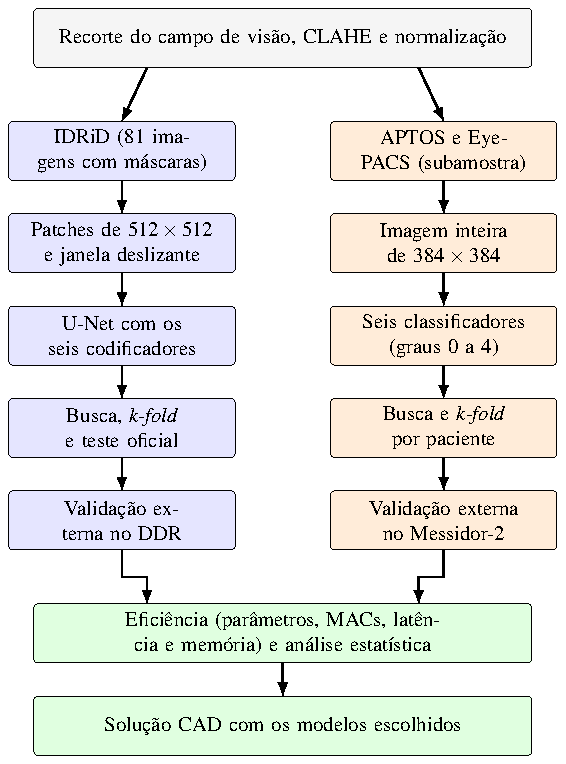
\includegraphics[width=9cm]{figuras/fig-met-geral}
	}{
		\Fonte{elaborada pelo autor.}
	}
\end{figure}

As imagens das duas tarefas passam pelo mesmo pré-processamento e depois seguem por ramos separados, já que a segmentação precisa da imagem em alta resolução e de máscaras de pixels, enquanto a classificação usa a imagem inteira em uma resolução menor e apenas o grau da doença como rótulo. Em cada ramo, os seis codificadores (VGG16, ResNet50, MobileNetV3-Large, EfficientNet-B0, ViT-B/16 e Swin-T) serão treinados nas mesmas condições, com a mesma divisão dos dados, o mesmo espaço de busca de hiperparâmetros e as mesmas métricas, de forma a deixar a arquitetura como a principal diferença entre os modelos.

As bases usadas para avaliar a generalização, DDR na segmentação e Messidor-2 na classificação, ficarão fora de qualquer etapa de treino, de escolha de hiperparâmetros ou de escolha de limiar, sendo consultadas uma única vez com os modelos finais. O mesmo vale para as 27 imagens de teste oficiais do IDRiD. Assim, evita-se o vazamento de informação discutido na Seção~\ref{sec:validacao} \cite{kapoor2023leakage}. Depois dos testes, os resultados de desempenho serão cruzados com as medidas de custo computacional, e os modelos escolhidos vão compor a solução CAD.

\section{Bases de dados}
\label{sec:bases-de-dados}

O trabalho utilizará cinco bases públicas de retinografias, duas para a segmentação e três para a classificação. A Tabela~\ref{tab:bases-resumo} resume o papel de cada uma no protocolo e as suas principais características.

\begin{table}[H]
	\caption{\label{tab:bases-resumo} Bases de dados e papel de cada uma no protocolo}%
	\IBGEtab{}{%
		\footnotesize
		\setlength{\tabcolsep}{4pt}\begin{tabular}{lp{2.1cm}p{2.5cm}p{2.3cm}p{2.5cm}p{2.1cm}}
			\toprule
			Base & Tarefa & Papel & Imagens usadas & Resolução e origem & Rótulos \\
			\midrule
			IDRiD & Segmentação & Desenvolvimento e teste & 81 (54 treino, 27 teste) & $4288 \times 2848$, Índia & Máscaras de EX e SE \\
			DDR & Segmentação & Validação externa & 225 (teste oficial) & 1088 a 5184 pixels, China & Máscaras de EX e SE \\
			APTOS 2019 & Classificação & Desenvolvimento & 3.662 antes da deduplicação & 474 a 4288 pixels, Índia & Graus 0 a 4 \\
			EyePACS & Classificação & Desenvolvimento & Subamostra de cerca de 10.000 & Variada, Estados Unidos & Graus 0 a 4 \\
			Messidor-2 & Classificação & Validação externa & 1.744 & 1440 a 2304 pixels, França & Graus 0 a 4 e edema adjudicados \\
			\bottomrule
		\end{tabular}%
	}{%
		\Fonte{elaborada pelo autor com dados de \citeonline{porwal2018idrid}, \citeonline{li2019ddr}, \citeonline{aptos2019}, \citeonline{eyepacs2015}, \citeonline{boumeshed2026modular} e \citeonline{krause2018grader}.}%
	}
\end{table}

\subsection{Bases para segmentação}
\label{sec:bases-segmentacao}

O IDRiD (\textit{Indian Diabetic Retinopathy Image Dataset}) é a base de desenvolvimento da segmentação. A parte com anotação de pixels tem 81 imagens com sinais de RD, obtidas com a câmera Kowa VX-10$\alpha$ com campo de 50° e pupila dilatada, em Nanded, na Índia, todas com $4288 \times 2848$ pixels \cite{porwal2018idrid}. Todas as 81 imagens têm máscara de exsudatos duros, mas só 40 têm máscara de exsudatos moles, e a divisão oficial separa 54 imagens para treino e 27 para teste, ficando 26 imagens com exsudatos moles no treino e 14 no teste. Essa divisão oficial será mantida, com o conjunto de teste usado apenas no fim, o que também permite comparar os resultados com os do desafio do IDRiD, que usou a AUPR como métrica \cite{porwal2020idrid}.

A base também traz marcações do centro do disco óptico e da fóvea em 516 imagens (413 de treino e 103 de teste) e máscaras do disco óptico nas 81 imagens, aproveitadas na solução CAD (Seção~\ref{sec:sistema-cad}). As imagens do IDRiD não têm identificador de paciente, então não há como garantir que os dois olhos de uma mesma pessoa fiquem no mesmo \textit{fold}, o que é assumido como uma limitação.

A DDR entra como base externa de segmentação. Ela foi coletada em 147 hospitais de 23 províncias da China, com 42 modelos de câmera, e a parte com anotação de lesões tem 757 imagens, sendo 486 com exsudatos duros e 239 com exsudatos moles, já divididas em 383 para treino, 149 para validação e 225 para teste \cite{li2019ddr}. Neste trabalho, apenas as 225 imagens de teste serão usadas, sem nenhum treino ou ajuste nessa base. Como as resoluções vão de $1088 \times 1920$ até $3456 \times 5184$ pixels, as imagens da DDR serão redimensionadas para que o diâmetro do campo de visão fique próximo ao das imagens do IDRiD, mantendo os exsudatos em uma escala parecida com a do treino.

\subsection{Bases para classificação}
\label{sec:bases-classificacao}

O APTOS 2019 tem 3.662 retinografias rotuladas de 0 a 4 segundo a escala ICDR, coletadas em clínicas da Índia \cite{aptos2019}. As imagens têm 17 tamanhos diferentes, com largura de 474 a 4288 pixels, e a base, assim como o IDRiD, não traz identificação de paciente, o que impede garantir que as duas imagens de uma mesma pessoa fiquem do mesmo lado da divisão \cite{boumeshed2026modular}. Outro problema é a presença de imagens quase duplicadas: \citeonline{boumeshed2026modular} encontraram 33 imagens do teste repetidas no treino ou na validação. Por isso, antes de qualquer divisão, as imagens serão comparadas por \textit{hash} perceptual, e os pares muito parecidos passarão por revisão, mantendo uma cópia quando o grau for o mesmo e descartando as duas quando os graus forem diferentes. A distribuição dos graus antes dessa limpeza aparece na Tabela~\ref{tab:dist-graus}.

\begin{table}[H]
	\caption{\label{tab:dist-graus} Distribuição dos graus no APTOS 2019 e no Messidor-2}%
	\IBGEtab{}{%
		\begin{tabular}{llrr}
			\toprule
			Grau & Descrição & APTOS 2019 & Messidor-2 \\
			\midrule
			0 & Sem RD aparente & 1.805 & 1.017 \\
			1 & RDNP leve & 370 & 270 \\
			2 & RDNP moderada & 999 & 347 \\
			3 & RDNP grave & 193 & 75 \\
			4 & RD proliferativa & 295 & 35 \\
			\midrule
			Total & & 3.662 & 1.744 \\
			\bottomrule
		\end{tabular}%
	}{%
		\Fonte{elaborada pelo autor com dados de \citeonline{aptos2019} e \citeonline{googlebrain2018messidor2}.}%
	}
\end{table}

O EyePACS tem 35.126 imagens de treino rotuladas, com duas imagens por paciente (olho direito e esquerdo) e cerca de três quartos das imagens no grau 0, segundo o arquivo de rótulos da competição \cite{eyepacs2015}. Ele vai entrar no desenvolvimento por trazer outra população e outras câmeras, mas usar a base inteira deixaria cada treino algumas vezes mais caro. Por isso, como escolha de projeto, será sorteada uma subamostra fixa de cerca de 5.000 pacientes (aproximadamente 10.000 imagens), que vai incluir todos os pacientes cujo pior olho tem grau 3 ou 4, por esses graus terem poucos casos nas duas bases, e completar o restante de forma estratificada pelo pior grau. Essa escolha muda a proporção dos graus na parte do EyePACS usada no desenvolvimento, que passa a ter mais casos graves e proliferativos do que a triagem real. Por isso, as métricas internas no EyePACS não representam a distribuição encontrada na prática, principalmente as que dependem da prevalência, como o valor preditivo positivo e o F1. O APTOS vai entrar inteiro, só sem as duplicatas, e o Messidor-2 e o teste de gradação do IDRiD mantêm a sua distribuição original, então é nessas bases que o desempenho com a distribuição natural vai ser medido.

Como a base não tem um rótulo de qualidade, as imagens sem condição de leitura (muito escuras, fora de foco ou sem o FOV visível) serão descartadas antes do sorteio. Para isso, uma verificação automática de brilho e nitidez será aplicada a todo o conjunto, e a inspeção visual será feita apenas nas imagens que essa verificação marcar como duvidosas. O identificador de paciente que aparece no nome do arquivo permitirá manter os dois olhos sempre no mesmo \textit{fold}, e o conjunto de desenvolvimento da classificação ficará sendo a união do APTOS sem duplicatas com essa subamostra.

O Messidor-2 é a base externa da classificação. Ele tem 874 exames com 1.748 imagens, adquiridas na França com a câmera Topcon TRC NW6 com campo de 45° \cite{decenciere2014messidor, boumeshed2026modular}. A base é distribuída sem graus oficiais, então serão usados os graus adjudicados por um painel de três especialistas em retina segundo o protocolo de \citeonline{krause2018grader}, disponibilizados em um arquivo público que traz, para cada imagem, o grau de RD, a presença de edema macular referenciável (exsudatos duros a até um diâmetro de disco) e a graduabilidade \cite{googlebrain2018messidor2}. Nesse arquivo, 1.744 imagens são graduáveis e 151 delas têm edema macular referenciável. A Tabela~\ref{tab:dist-graus} mostra que o Messidor-2 tem bem menos casos graves e proliferativos que o APTOS, o que já indica uma mudança de distribuição entre o desenvolvimento e o teste externo.

\subsection{Aspectos éticos e licenças de uso}
\label{sec:etica-licencas}

Este trabalho não envolve coleta de dados com seres humanos nem contato com pacientes. Todas as imagens vêm de bases públicas (IDRiD, DDR, APTOS, EyePACS e Messidor-2), disponibilizadas pelos seus responsáveis para fins de pesquisa, já anonimizadas e sem nenhuma informação que permita identificar os pacientes. Por usar apenas informações de acesso público, sem identificação dos participantes, o trabalho se enquadra no art. 1º, parágrafo único, inciso II, da Resolução nº 510/2016 do Conselho Nacional de Saúde, que dispensa o registro e a avaliação pelo sistema CEP/Conep \cite{brasil2016res510}. Os termos de uso de cada base serão respeitados, como a licença \textit{Creative Commons Attribution} do IDRiD e as regras das competições do Kaggle no caso do APTOS e do EyePACS, e as imagens não serão redistribuídas.

\section{Pré-processamento}
\label{sec:met-preprocessamento}

O pré-processamento é o mesmo para todas as bases e para as duas tarefas, com exceção do tamanho final da imagem. O campo de visão (FOV, do inglês \textit{Field of View}) será detectado por um limiar simples no canal vermelho, e a imagem será recortada ao menor retângulo que o contém, retirando a borda preta que varia muito entre câmeras. Sobre a imagem recortada, será aplicado o CLAHE \cite{pizer1987ahe} no canal L do espaço de cor CIELAB, com limite de recorte 2,0 e grade de $8 \times 8$ blocos. Isso melhora o contraste local sem mudar a cor da imagem, seguido da normalização dos valores com a média e o desvio padrão do ImageNet, já que todos os codificadores partem de pesos pré-treinados nessa base. Para reduzir o tempo de leitura das imagens grandes durante o treino, as imagens recortadas e equalizadas de todas as bases serão salvas em disco uma única vez antes do treino, já no tamanho final no caso da classificação.

Na segmentação, a imagem do IDRiD será mantida na resolução original depois do recorte, pois os exsudatos podem ter poucos pixels e uma redução para $224 \times 224$ apagaria boa parte deles. O treino vai usar recortes (\textit{patches}) de $512 \times 512$ pixels e a predição será feita na imagem inteira por janela deslizante, como descrito na Seção~\ref{sec:protocolo-seg}, prática que também aparece em \citeonline{zong2020unet}, que extraíram os \textit{patches} das imagens originais. As máscaras de EX e SE serão empilhadas em dois canais binários, e qualquer redimensionamento de máscara vai usar vizinho mais próximo, para não criar valores intermediários.

Na classificação, a imagem recortada será redimensionada para $384 \times 384$ pixels, mantendo a proporção e completando com preto quando necessário. \citeonline{sahlsten2019} mostraram que a gradação melhora com resoluções maiores que a usual de $224 \times 224$, e o valor de 384 foi escolhido por caber na memória da GPU disponível para os seis modelos. Se o orçamento permitir, o melhor modelo convolucional e o melhor \textit{Transformer} também serão treinados com 512 pixels, para medir quanto a resolução muda o resultado.

\section{Arquiteturas}
\label{sec:met-arquiteturas}

Os seis codificadores são os apresentados na Seção~\ref{sec:ft-arquiteturas}, todos com pesos pré-treinados no ImageNet. Na classificação, a saída do codificador passa por uma média global (ou pelo \textit{token} de classe, no caso do ViT), por uma camada de \textit{dropout} e por uma camada linear com cinco saídas, uma por grau. Na segmentação, todos os codificadores são ligados ao mesmo decodificador U-Net \cite{ronneberger2015unet}, que recebe mapas de características em quatro escalas (1/4, 1/8, 1/16 e 1/32 do tamanho da entrada). Para recuperar os detalhes finos, um pequeno bloco convolucional igual para todos os modelos processa a própria imagem na escala 1/2 e fornece a conexão de salto mais rasa. A forma como cada codificador entrega essas quatro escalas está na Tabela~\ref{tab:encoders}.


Os codificadores convolucionais e o Swin-T já são hierárquicos, então basta ler os mapas no fim de cada estágio. O ViT-B/16 é o único caso que precisa de adaptação, pois todos os seus blocos trabalham na mesma escala. Seguindo a ideia da UNETR \cite{hatamizadeh2022unetr}, proposta para volumes 3D e aqui adaptada para 2D, os \textit{tokens} dos blocos 3, 6, 9 e 12 são reorganizados em mapas de $32 \times 32$ e levados às quatro escalas por convoluções transpostas (para 1/4 e 1/8), por uma projeção simples (para 1/16) e por uma convolução com passo 2 (para 1/32).

\begin{table}[H]
	\caption{\label{tab:encoders} Ligação de cada codificador ao decodificador U-Net}%
	\IBGEtab{}{%
		\footnotesize
		\begin{tabular}{lp{9.6cm}}
			\toprule
			Codificador & Mapas usados nas conexões de salto \\
			\midrule
			VGG16 & Saídas dos blocos 2 a 5 depois de cada \textit{max pooling} (1/4, 1/8, 1/16 e 1/32) \\
			ResNet50 & Saídas dos estágios conv2\_x a conv5\_x \\
			MobileNetV3-Large & Saídas dos blocos em que a resolução cai para 1/4, 1/8, 1/16 e 1/32 \\
			EfficientNet-B0 & Saídas dos estágios em que a resolução cai para 1/4, 1/8, 1/16 e 1/32 \\
			ViT-B/16 & \textit{Tokens} dos blocos 3, 6, 9 e 12 (escala 1/16), reorganizados em mapas e reamostrados para 1/4, 1/8, 1/16 e 1/32, no estilo da UNETR \\
			Swin-T & Saídas dos quatro estágios, já em 1/4, 1/8, 1/16 e 1/32 \\
			\bottomrule
		\end{tabular}%
	}{%
		\Fonte{elaborada pelo autor.}%
	}
\end{table}

Como o ViT foi pré-treinado com entradas de $224 \times 224$, ou $14 \times 14$ \textit{patches}, os \textit{embeddings} de posição serão interpolados de forma bidimensional para a grade de $32 \times 32$ das entradas de 512 pixels, e para $24 \times 24$ na classificação com 384 pixels, como \citeonline{dosovitskiy2021vit} fazem no ajuste fino em resolução maior. O Swin-T não tem \textit{embedding} de posição absoluto, e o seu viés de posição relativa depende só do tamanho da janela, que continua o mesmo, de modo que ele pode receber entradas de 512 pixels com o preenchimento necessário para que o mapa seja múltiplo da janela, como no uso do Swin em segmentação com entradas de $512 \times 512$ \cite{liu2021swin}.

A saída do decodificador tem dois canais, um para exsudatos duros e outro para exsudatos moles, cada um com a sua própria função sigmoide, porque cada lesão tem a sua própria máscara binária no IDRiD e na DDR, e um pixel pode ser marcado em mais de uma delas. Os canais do decodificador (256, 128, 64, 32 e 16, da escala mais funda para a mais rasa) são os mesmos em todos os modelos, de forma que a diferença de parâmetros entre eles venha do codificador. Como o lote real das redes maiores com \textit{patches} de 512 pixels fica pequeno, o decodificador usa normalização de grupo (\textit{GroupNorm}) no lugar da normalização em lote, e as camadas de normalização em lote do codificador ficam congeladas, em modo de avaliação, sempre que o lote real tiver menos de 8 amostras. Como o lote real depende do tamanho de cada rede, esse critério faz com que algumas redes tenham a normalização em lote congelada e outras não, o que será registrado como uma limitação do protocolo na análise dos resultados.

\section{Protocolo experimental}
\label{sec:protocolo-experimental}

O protocolo busca responder a duas perguntas sem aumentar demais o custo: qual configuração de treino cada arquitetura deve usar e quão estável é o desempenho dessa configuração. Por isso, a busca de hiperparâmetros será feita uma única vez, em uma divisão fixa, e apenas a melhor configuração de cada arquitetura passará pela validação cruzada completa.

\subsection{Particionamento dos dados}
\label{sec:particionamento}

Na segmentação, as 54 imagens de treino do IDRiD serão divididas em 5 \textit{folds} estratificados pela presença de exsudatos moles, para que todo \textit{fold} tenha imagens com SE, e essa divisão será repetida 3 vezes com sementes diferentes, totalizando 15 rodadas pareadas por arquitetura. As 27 imagens de teste oficiais não entram em nenhum \textit{fold}. Na classificação, o conjunto de desenvolvimento será dividido em 5 \textit{folds} com \textit{StratifiedGroupKFold}, em que o grupo é o paciente no EyePACS e cada imagem já deduplicada no APTOS, com estratificação pelo grau e 2 repetições, totalizando 10 rodadas.

Em todas as rodadas, o \textit{fold} de avaliação ficará separado, e o critério de parada antecipada vai usar uma validação interna retirada dos \textit{folds} de treino (cerca de 15\% das imagens, com a mesma estratificação e o mesmo agrupamento). Assim, o \textit{fold} de avaliação não participa de nenhuma decisão de treino, evitando a estimativa otimista que ocorre quando a mesma partição escolhe e avalia o modelo \cite{varma2006bias, cawley2010overfitting}. As divisões serão sorteadas uma única vez, salvas em arquivos e usadas por todos os modelos.

\subsection{Aumento de dados}
\label{sec:da-comum}

O aumento de dados será aplicado só no treino, com as mesmas transformações para todos os modelos de uma tarefa: inversões horizontal e vertical, rotações de até 30°, pequenas variações de escala e de translação, e mudanças leves de brilho, contraste e saturação. Na segmentação, as transformações geométricas valerão também para as máscaras, com interpolação por vizinho mais próximo. Transformações que mudam muito a cor vão ficar de fora, já que a cor amarelada ou esbranquiçada é um dos sinais que separa os exsudatos das outras estruturas.

\subsection{Busca de hiperparâmetros}
\label{sec:busca-hiperparametros}

A busca é uma busca em grade pequena, mostrada na Tabela~\ref{tab:grid-search}, feita em uma divisão fixa. Na segmentação, as 54 imagens de treino do IDRiD serão separadas em 43 para treino e 11 para validação, estratificadas pela presença de SE, sem usar nenhuma imagem do teste oficial. Na classificação, será usada uma divisão de 80\% e 20\% do conjunto de desenvolvimento, agrupada por paciente. O critério de escolha é a métrica principal na validação, a AUPR média de EX e SE na segmentação e o QWK na classificação. Como a grade tem poucos valores, ela foi preferida à busca aleatória, que é mais vantajosa quando há muitos hiperparâmetros e só alguns importam \cite{bergstra2012random}. Como a busca e a validação cruzada usam o mesmo conjunto de desenvolvimento, as médias da validação cruzada podem ficar um pouco otimistas para a configuração escolhida, e a estimativa sem esse viés é a do teste oficial do IDRiD e a das bases externas.

\begin{table}[H]
	\caption{\label{tab:grid-search} Espaço de busca de hiperparâmetros}%
	\IBGEtab{}{%
		\begin{tabular}{lll}
			\toprule
			Hiperparâmetro & Segmentação & Classificação \\
			\midrule
			Taxa de aprendizado & $3 \times 10^{-4}$, $10^{-4}$, $3 \times 10^{-5}$ & $3 \times 10^{-4}$, $10^{-4}$, $3 \times 10^{-5}$ \\
			Otimizador & Adam, AdamW & Adam, AdamW \\
			Ajuste fino & Total & Total, parcial \\
			\midrule
			Configurações por arquitetura & 6 & 12 \\
			\bottomrule
		\end{tabular}%
	}{%
		\Fonte{elaborada pelo autor.}%
	}
\end{table}

O tamanho do lote não entra na grade. Com 8 GB de memória, o ViT-B/16 não comporta lotes grandes de \textit{patches} de 512 pixels, e variar o lote junto com a taxa de aprendizado deixaria arquiteturas diferentes com buscas diferentes. Por isso, cada modelo vai usar o maior lote que couber na memória e o acúmulo de gradientes até um lote efetivo de 16 \textit{patches} na segmentação e 32 imagens na classificação, e o lote real de cada rede será informado nos resultados. Os otimizadores Adam \cite{kingma2015adam} e AdamW \cite{loshchilov2019adamw} usam um aquecimento linear da taxa de aprendizado nas primeiras épocas, que ajuda a estabilizar o ajuste fino dos \textit{Transformers}, seguido de decaimento por cosseno, e o AdamW usa decaimento de pesos de 0,01. No ajuste fino parcial, ficam congelados os dois primeiros estágios nas redes convolucionais e no Swin-T, e a projeção dos \textit{patches} e os quatro primeiros blocos no ViT-B/16.

\subsection{Treinamento}
\label{sec:protocolo-treino}

\subsubsection{Segmentação}
\label{sec:protocolo-seg}

Cada época de segmentação terá 500 \textit{patches} de $512 \times 512$ sorteados das imagens de treino. Metade deles vai ser centrada em um pixel de lesão escolhido ao acaso, com mais peso para os exsudatos moles por serem mais raros, e a outra metade será sorteada em qualquer ponto do FOV, para que a rede também veja regiões sem lesão. A perda é a soma da entropia cruzada binária com a perda Dice, calculadas para cada canal e somadas, combinação que se mostrou estável em vários problemas de segmentação \cite{ma2021loss}. A perda Dice é calculada sobre o lote inteiro e com um pequeno termo de suavização, de modo que um lote sem exsudato mole não gere uma divisão por zero.

Na validação e no teste, a predição será feita na imagem inteira por janela deslizante, com janelas de $512 \times 512$ e sobreposição de metade da janela, combinando as janelas com pesos que diminuem do centro para a borda, como no nnU-Net \cite{isensee2021nnunet}. Na segmentação, a validação interna é feita por janela deslizante sobre as imagens inteiras, um processo bem mais lento que o treino em recortes. Por isso, ela será executada a cada 5 épocas, e não ao final de cada época, e a parada antecipada considera 15 épocas sem melhora (três validações seguidas). Esse intervalo é uma escolha deste trabalho para reduzir o custo do treino e será conferido no treino piloto, podendo ser reduzido se o tempo de GPU permitir. O treino terá no máximo 100 épocas, a melhora será medida pela AUPR média da validação interna, e serão guardados os pesos da melhor validação.

\subsubsection{Classificação}
\label{sec:protocolo-clf}

Na configuração principal, a classificação será tratada como um problema de cinco classes com entropia cruzada ponderada pelo inverso da frequência de cada grau, para compensar o excesso de imagens no grau 0. Como os graus são ordenados, a entropia cruzada não penaliza mais um erro de 0 para 4 do que um erro de 0 para 1, e por isso o QWK é a métrica de escolha. Para o melhor modelo, serão testadas também duas alternativas ordinais: tratar o grau como regressão, com os limiares entre as classes escolhidos na validação, e treinar com a perda baseada no kappa ponderado de \citeonline{delatorre2018kappa}. O treino terá no máximo 30 épocas, com parada antecipada se o QWK da validação interna não melhorar em 5 épocas.

A probabilidade de RD referenciável sai do mesmo modelo de cinco classes, somando as probabilidades dos graus 2, 3 e 4, sem precisar de outro modelo binário. Aqui a RD referenciável é definida só pelo grau (moderada ou pior), já que o APTOS e o EyePACS não trazem rótulos de edema macular.

\subsubsection{Escolha e modelo final de cada arquitetura}
\label{sec:modelo-final}

A validação cruzada serve para estimar o desempenho e a sua variação, mas os 15 ou 10 modelos das rodadas não vão para o teste. Para cada arquitetura, a configuração escolhida será treinada de novo com todo o conjunto de desenvolvimento (as 54 imagens do IDRiD ou todo o APTOS e a subamostra do EyePACS), pelo número de épocas igual à mediana das melhores épocas da validação cruzada. Esse modelo único será o avaliado no teste oficial do IDRiD e nas bases externas, com os limiares de decisão iguais às médias dos limiares escolhidos nas validações das rodadas.

Sempre que o texto fala do melhor modelo de uma tarefa, como nos testes com 512 pixels, nas alternativas ordinais e na solução CAD, trata-se do modelo com a maior média da métrica principal na validação cruzada. Entre modelos sem diferença significativa, fica o de menor latência. O teste oficial do IDRiD e as bases externas não entram nessa escolha.

\section{Métricas de avaliação}
\label{sec:met-metricas}

Na segmentação, as métricas são calculadas para cada lesão em separado, apenas dentro do FOV. A métrica principal é a AUPR (área sob a curva de precisão e revocação), que não depende de limiar e é a métrica do desafio IDRiD \cite{porwal2020idrid}. O coeficiente Dice (DSC) é a segunda métrica principal e o IoU é complementar, com os verdadeiros positivos, falsos positivos e falsos negativos somados sobre todas as imagens do conjunto, de forma que uma imagem sem exsudato mole não gere o caso 0/0 sozinha. O limiar usado no Dice e no IoU será escolhido na validação. A acurácia e a especificidade de pixel não entram na comparação, porque o fundo domina a imagem e deixa esses valores perto de 1 para qualquer modelo.

Na classificação, a métrica principal é o QWK (\textit{Quadratic Weighted Kappa}) \cite{cohen1968kappa}, que leva em conta a distância entre o grau previsto e o real. A segunda métrica principal é a AUC da RD referenciável, calculada com a probabilidade somada dos graus 2 a 4, acompanhada da sensibilidade e da especificidade em um ponto de operação, do F1 macro e da matriz de confusão dos cinco graus. O limiar desse ponto de operação será escolhido na validação interna de cada modelo, pelo índice de Youden (o valor que maximiza a soma da sensibilidade e da especificidade), e ficará fixo antes de qualquer avaliação no teste e nas bases externas.

O custo de cada modelo será medido pelo número de parâmetros, pelos MACs, definidos na Seção~\ref{sec:metricas-eficiencia}, pela latência e pelo pico de memória. Os MACs das seis redes serão contados com a mesma ferramenta, a biblioteca fvcore, que conta cada multiplicação-soma como uma operação, na mesma resolução de entrada usada em cada tarefa ($512 \times 512$ na segmentação e $384 \times 384$ na classificação). A latência será medida com lote de tamanho 1, na GPU e na CPU, como a mediana de 100 execuções depois de 20 execuções de aquecimento, e, na segmentação, também a latência da imagem inteira por janela deslizante. Esses valores serão cruzados com o desempenho na escolha dos modelos da solução CAD (Seção~\ref{sec:sistema-cad}).

\section{Validação externa}
\label{sec:validacao-externa}

Os modelos finais da Seção~\ref{sec:modelo-final} serão aplicados na DDR e no Messidor-2 sem nenhum ajuste, mantendo o pré-processamento e os limiares escolhidos no desenvolvimento. Essa avaliação mostra quanto do desempenho se mantém em outra população, com outras câmeras e outros avaliadores. Uma queda grande é esperada: \citeonline{boumeshed2026modular} treinaram um classificador no APTOS e viram o QWK cair de 0,873 no teste do APTOS para 0,455 no Messidor-2. Na DDR, parte da queda também pode vir de diferenças no protocolo de anotação entre as bases, e não apenas do modelo. Por isso, os resultados externos vão aparecer ao lado dos internos e serão analisados como uma medida de generalização.

\section{Análise estatística}
\label{sec:analise-estatistica}

Para cada métrica principal, as seis arquiteturas serão comparadas duas a duas, totalizando 15 pares. Na validação cruzada, cada par passará por dois testes, aplicados aos valores pareados de cada rodada, que são 15 na segmentação (5 \textit{folds} $\times$ 3 repetições) e 10 na classificação (5 \textit{folds} $\times$ 2 repetições). O primeiro é o teste de Wilcoxon pareado \cite{wilcoxon1945}, bilateral, com valor-p exato, ou com a aproximação normal quando houver empates entre as diferenças. O segundo é o teste \textit{t} corrigido de \citeonline{nadeau2003inference}, que aumenta a variância estimada para levar em conta a sobreposição dos conjuntos de treino entre as rodadas, usando as $J = 15$ rodadas da segmentação e as $J = 10$ da classificação, com $J - 1$ graus de liberdade (14 e 9) e razão de cerca de 0,29 entre o tamanho do \textit{fold} de avaliação e o da parte efetivamente usada no treino (20\% contra 68\%, já descontados os 15\% reservados para a validação interna). Os valores-p dos 15 pares passarão pelo ajuste de \citeonline{holm1979simple}, separadamente para cada teste, com nível de significância de 5\%. Cada família do ajuste é formada pelos 15 pares de uma mesma métrica principal em um mesmo conjunto de avaliação (validação cruzada, teste do IDRiD, DDR ou Messidor-2). Como há mais de uma família, o controle do erro vale dentro de cada uma, e não para o conjunto de todos os testes. Os dois testes serão lidos em conjunto. Uma diferença entre dois modelos será tratada como consistente quando os dois testes, depois do ajuste de Holm, apontarem significância no mesmo sentido. Quando só um deles apontar diferença, o resultado será relatado como inconclusivo e discutido junto com o tamanho da diferença. Com tão poucos valores pareados, o Wilcoxon tem pouco poder. Na classificação, com 10 rodadas, o menor valor-p possível é cerca de 0,002, abaixo do limiar de $0{,}05/15 \approx 0{,}0033$ do primeiro passo do Holm, mas isso só acontece quando um modelo vence o outro em todas as rodadas. Por isso, a falta de significância não será lida como empate entre os modelos.

O teste de Friedman e o pós-teste de Nemenyi \cite{demsar2006statistical} servem só para ordenar os modelos e desenhar o diagrama de diferença crítica, de forma descritiva, porque as rodadas não são independentes.

Nos conjuntos de teste fixos, o teste oficial do IDRiD, a DDR e o Messidor-2, o intervalo de confiança de 95\% da diferença entre dois modelos vem de um \textit{bootstrap} pareado com 1.000 reamostragens \cite{efron1979bootstrap}. No Messidor-2, a reamostragem será feita por exame, e não por imagem, já que cada exame tem duas imagens do mesmo paciente. No Messidor-2, o intervalo da diferença de AUC da RD referenciável também virá desse \textit{bootstrap} por exame. O teste de \citeonline{delong1988}, com o mesmo ajuste de Holm, será apresentado apenas como complemento, porque supõe imagens independentes, o que não ocorre quando os dois olhos de um exame entram na análise. Como o teste do IDRiD tem só 27 imagens, e apenas 14 com exsudatos moles, os intervalos nessa base devem ser largos, e uma diferença sem significância ali não será interpretada como empate.

\section{Ambiente computacional e reprodutibilidade}
\label{sec:ambiente-computacional}

O plano é executar os experimentos em um computador com GPU NVIDIA GeForce RTX 4060 Ti de 8 GB, processador AMD Ryzen 7 5700X e 16 GB de memória RAM, o mesmo usado para medir a latência. Para caber nessa memória, o treino usa precisão mista e, nos \textit{Transformers} com entrada de 512 pixels, \textit{checkpointing} de gradientes. A implementação é feita em Python com PyTorch, com os codificadores e os pesos pré-treinados da biblioteca timm, o decodificador U-Net implementado pelo autor e bibliotecas de apoio como Albumentations, scikit-learn, fvcore e Streamlit. As versões exatas das bibliotecas, os nomes dos pesos pré-treinados e as divisões dos dados ficam salvos junto com o código, e cada repetição usa uma semente fixa para a divisão, a inicialização e o sorteio dos \textit{patches}.

A Tabela~\ref{tab:orcamento} estima o custo de treinamento. O custo varia bastante entre as redes, já que a VGG16 e o ViT-B/16 a 512 pixels custam várias vezes mais que as redes leves, e por isso as horas da tabela são médias por treino e o total deve ser lido como uma ordem de grandeza, entre 150 e 300 horas de GPU, a ser confirmada no início da execução com um treino piloto da ResNet50 e do ViT-B/16 em cada tarefa. São 272 treinos no plano principal, cerca de um quinto dos aproximadamente 1.260 que seriam necessários repetindo a mesma grade em todos os \textit{folds}. Os experimentos extras da classificação, com as alternativas ordinais e a entrada de 512 pixels, somam outros 44 treinos (cerca de 62 horas) e ficam fora do total, rodando só se sobrar tempo.

\begin{table}[H]
	\caption{\label{tab:orcamento} Estimativa do número de treinos e de horas de GPU}%
	\IBGEtab{}{%
		\begin{tabular}{llrrr}
			\toprule
			Tarefa & Etapa & Treinos & \begin{tabular}[b]{@{}r@{}}Horas por treino\\(média estimada)\end{tabular} & Horas de GPU \\
			\midrule
			Segmentação & Busca ($6 \times 6$) & 36 & 0,4 & 14 \\
			Segmentação & Validação cruzada ($6 \times 15$) & 90 & 0,5 & 45 \\
			Segmentação & Modelos finais & 6 & 0,6 & 4 \\
			Classificação & Busca ($6 \times 12$) & 72 & 0,6 & 43 \\
			Classificação & Validação cruzada ($6 \times 10$) & 60 & 1,0 & 60 \\
			Classificação & Modelos finais & 6 & 1,2 & 7 \\
			CAD & Disco óptico e fóvea & 2 & 2,0 & 4 \\
			\midrule
			Total do plano principal & & 272 & & 177 \\
			\midrule
			Classificação (opcional) & Ordinal e 512 pixels & 44 & 1,4 & 62 \\
			\bottomrule
		\end{tabular}%
	}{%
		\Fonte{elaborada pelo autor.}%
	}
\end{table}

Caso o piloto mostre um custo bem maior que o estimado, o plano será reduzido nesta ordem: usar 2 repetições em vez de 3 na segmentação, tirar o ajuste fino parcial da busca da classificação, diminuir a subamostra do EyePACS ou deixá-la de fora, ficando só com o APTOS. Se ainda faltar tempo, a validação cruzada dos \textit{Transformers} vai ser feita em GPUs gratuitas do Kaggle ou do Google Colab, ou em horas de GPU alugadas em nuvem. Qualquer redução valerá igualmente para os seis modelos e será informada nos resultados.

\section{Solução CAD}
\label{sec:sistema-cad}

A solução CAD vai reunir o melhor modelo de segmentação e o melhor modelo de classificação, escolhidos pelo desempenho e pelo custo, em uma aplicação web feita com Streamlit, cujo fluxo é mostrado na Figura~\ref{fig:fluxo-cad}. O usuário envia uma retinografia, que passa pelo mesmo pré-processamento do desenvolvimento, e a imagem segue ao mesmo tempo para o segmentador, que gera as máscaras de exsudatos duros e moles, e para o classificador, que gera o grau previsto e a probabilidade de RD referenciável.

\begin{figure}[!t]
	\centering
	\Caption{\label{fig:fluxo-cad} Fluxo da solução CAD}
	\UFCfig{}{
		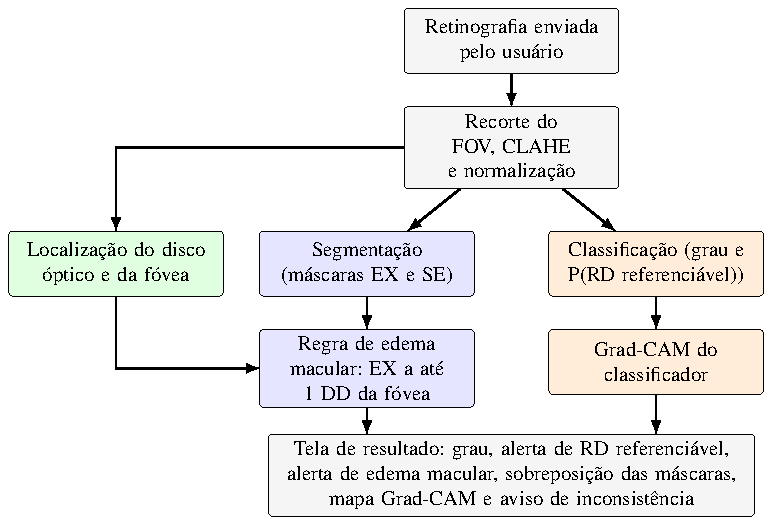
\includegraphics[width=14cm]{figuras/fig-met-cad}
	}{
		\Fonte{elaborada pelo autor.}
	}
\end{figure}

A integração entre os dois módulos se dá pela regra de edema macular da Seção~\ref{sec:cad}: se houver exsudatos duros a até um diâmetro de disco (DD) do centro da fóvea, a imagem é marcada como suspeita de edema macular referenciável \cite{krause2018grader}. Para que um único pixel falso positivo não dispare o alerta, um exsudato duro só será considerado quando a probabilidade prevista passar de um limiar e a região conectada tiver uma área mínima, e os dois valores serão escolhidos com as imagens de treino do IDRiD, antes de qualquer avaliação da regra. Para localizar a fóvea e o disco, a solução tem dois modelos auxiliares, fora da comparação principal e com uma configuração fixa.

O disco óptico será segmentado por uma U-Net com codificador ResNet50, treinada com as máscaras de disco das 54 imagens de treino do IDRiD, e o diâmetro do disco corresponde ao diâmetro do círculo de mesma área da máscara prevista. O centro da fóvea será localizado pela mesma arquitetura com um canal de saída que prevê um mapa de calor gaussiano em torno do ponto, treinada com as 413 marcações de fóvea do treino do IDRiD \cite{porwal2018idrid}. Os dois modelos serão avaliados nos conjuntos de teste do IDRiD, pelo Dice no disco e pela distância entre a fóvea prevista e a marcada, medida em diâmetros de disco. Como um erro na fóvea muda o resultado da regra, a interface vai mostrar o ponto encontrado e permitir que o usuário o corrija.

A regra será avaliada em duas bases. A primeira são as 103 imagens de teste de gradação do IDRiD, em que o risco de edema macular segue as definições do Messidor \cite{porwal2018idrid}: risco 0 quando não há exsudatos duros visíveis, risco 1 quando a menor distância entre a mácula e os exsudatos duros é maior que um diâmetro de papila e risco 2 quando essa distância é de até um diâmetro de papila \cite{adcis2008messidor}. O diâmetro de papila é o mesmo diâmetro do disco óptico usado na regra. A regra será considerada positiva para o risco 2 e negativa para os riscos 0 e 1. Antes disso, as imagens desse teste que também estiverem no treino da segmentação serão encontradas por \textit{hash} perceptual e retiradas dessa avaliação. A segunda são as 1.744 imagens graduáveis do Messidor-2, comparando a regra com a coluna de edema macular referenciável adjudicado, que usa o mesmo critério de um diâmetro de disco \cite{googlebrain2018messidor2}. Para essa avaliação, as imagens do Messidor-2 serão redimensionadas da mesma forma que as da DDR, pelo diâmetro do campo de visão, para que os exsudatos e o disco tenham tamanho parecido com o das imagens do IDRiD. Nas duas bases, a regra terá a sua sensibilidade e a sua especificidade informadas.

A tela de resultado vai mostrar o grau previsto com as probabilidades, o alerta de RD referenciável, o alerta de edema macular, as máscaras sobre a imagem e o mapa Grad-CAM do classificador \cite{selvaraju2017gradcam}. Quando os dois módulos discordarem, por exemplo com grau 0 previsto e exsudatos segmentados, a tela mostrará um aviso de inconsistência pedindo revisão. Neste trabalho, a segmentação não será usada como entrada do classificador, pois \citeonline{boumeshed2026modular} não encontraram melhora significativa na gradação ao juntar características das lesões à imagem, e a integração aqui proposta tem como ganho principal a explicação da decisão e o alerta de edema, informação que o classificador sozinho não fornece. A solução é pensada como uma ferramenta de apoio e não substitui a avaliação de um especialista, e a sua validação clínica fica fora do escopo deste trabalho.
